\documentclass{article}
\usepackage[utf8]{inputenc}
\usepackage{url}
\usepackage{amsmath,amsthm,enumitem}
\usepackage{graphicx}
\usepackage{lscape}
\usepackage{geometry}
\usepackage{color}
\usepackage{float}
\usepackage{listings}
\usepackage{amssymb}
\usepackage{enumitem}
\usepackage{verbatim}
\usepackage{algpseudocode} 
\usepackage{algorithm}  
\usepackage{algorithmicx}  
\usepackage{hyperref}
\geometry{left=2.5cm,right=2.5cm,top=2.5cm,bottom=2.5cm} 
\renewcommand{\baselinestretch}{1.5}
\setcounter{MaxMatrixCols}{20}

\title{Note on Adaptive Riemannian Metrics}
\author{Haocheng Dai }
\date{\today}
\theoremstyle{definition}
\newtheorem{definition}{Definition}
\theoremstyle{plain}
\newtheorem{theorem}{Theorem}
\newtheorem{lemma}{Lemma}
\DeclareUnicodeCharacter{2212}{-}
\begin{document}
\maketitle

\section{Mathematical Background}
\subsection{Riemannian Manifold}
\begin{definition} 
A \textbf{Riemannian manifold} is a differentiable manifold equipped with a Riemannian metric. 

In a differentiable manifold, each point has a neighborhood that is equivalent to the Euclidean space. In differential geometry, for each point $p$ on a manifold $M$, there is a vector space attached to each point. The vector space is called tangent space and is usually denoted as $T_pM$.
\end{definition}

\begin{definition}
A \textbf{Riemannian metric} on a differential manifold $M$ is a smooth function that associates to each point $p$ of $M$ an inner product $\langle\cdot,\cdot\rangle$ on the tangent space $T_pM$.
\end{definition}
The Riemannian metric can be equated with a smoothly varying positive-definite symmetric matrix $g$, called the metric tensor, defined at each point. For two vectors $v,w\in T_pM$, given local coordinates $(x^1, x^2,\cdots,x^n)$ in a neighborhood of $p$, the entry in $g$ ($n\times n$ matrix) can be expressed like below
\begin{equation*}
    g_{ij}=\langle E_i,E_j\rangle,
\end{equation*}
where $E_i=\frac{\partial}{\partial x^i}$ are the coordinate basis vectors at $p$.

With this definition, we can compute the inner product $\langle v,w\rangle$ as $v^Tgw$. Also, for a vector $v$, we can compute the length of the vector as $\langle v,v\rangle^\frac{1}{2}$, which is the $L^2$ norm.

Sometimes, people utilize the inverse of the diffusion tensor, $D^{-1}$, to define a local cost function as
\begin{equation*}
    \langle v,w\rangle=v^TD^{-1}w,
\end{equation*}
where $v, w\in T_pM$.

In this case, since the inverse of the diffusion tensor are positive-definite symmetric and they are also Riemannian metric, a DTI is actually wrapped into a Riemannian manifold.

The inverse tensor cost function makes sense, as shown in Figure 1. As we move in the major axis of the diffusion tensor, the time cost is low; as we move in the minor axis of the diffusion tensor, the cost is high.
\begin{figure}[H]
   \centering
   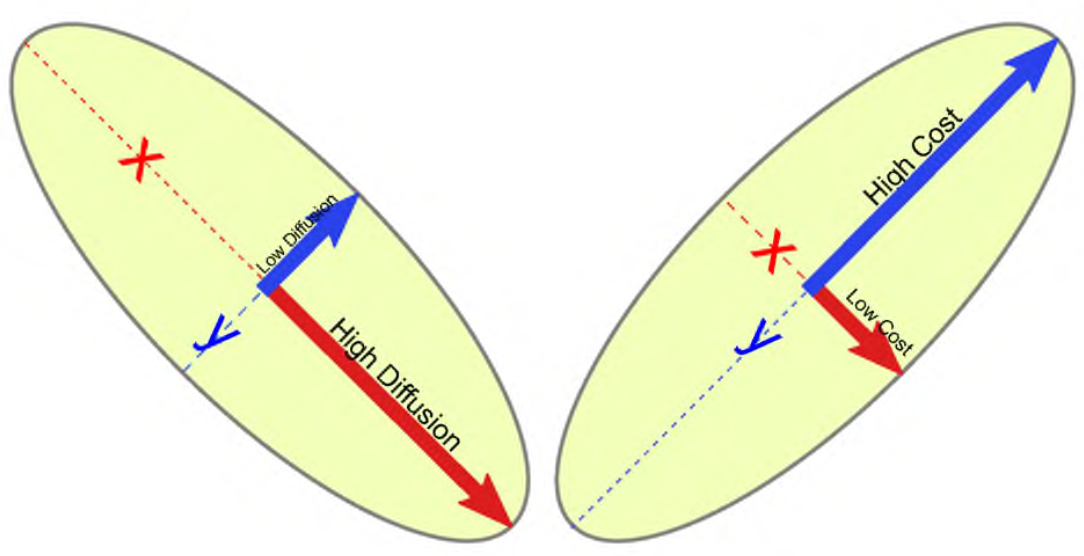
\includegraphics[scale=0.3]{figure/diffusion.png}
   \caption{Inverse diffusion tensor as Riemannian metric}
\end{figure}

To connect nearby tangent spaces (see Figure 2) on a Riemannian manifold, we need the Riemannian connection $\nabla_XY$, which is the derivative of a vector field $Y$ in the direction of a vector field $X$. The Riemannian connection is given by
\begin{equation*}
    \nabla_XY=\sum_k^n\left(\sum_i a^i\frac{\partial b^k}{\partial x^i}+\sum_{i,j}\Gamma_{ij}^k a^i b^j\right)\vec{E_k}
\end{equation*}
where $X=\sum a^iE_i$ and $Y=\sum b^jE_j$, $a^i$ and $b^j$ are smooth coefficient functions.

\begin{figure}[H]
   \centering
   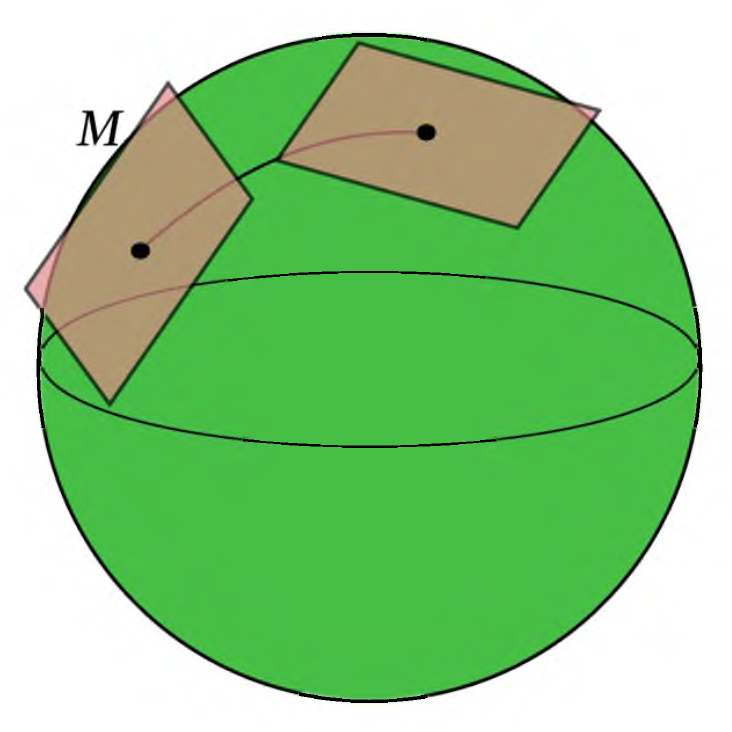
\includegraphics[scale=0.3]{figure/tangentspace.png}
   \caption{Tangent Space}
\end{figure}

\subsection{Geodesic on Riemannian Manifold}

On a Riemannian manifold $M$, the geodesic between two points $p,q\in M$ is defined by the minimization of the length functional
\begin{equation}
    u(\gamma)=\int^1_0\langle\Dot{\gamma}(t),\Dot{\gamma}(t)\rangle^\frac{1}{2}dt
\end{equation}
where $\gamma:[0,1]\rightarrow M$ is a curve with fixed endpoints $\gamma(0)=p, \gamma(1)=q$. The inner product between two tangent vectors $v,w\in T_xM$ is given by $\langle v,w\rangle=v^Tg(x)w$, where $g(x)$ is the Riemannian metric at point $x$.

Obviously, a critical curve for Eq.(1) is also a critical curve for
\begin{equation}
    E(\gamma)=\int^1_0\langle\Dot{\gamma}(t),\Dot{\gamma}(t)\rangle dt
\end{equation}
which is easier to work on. The only difference is that the geodesic that minimizes $E(\gamma)$ has a constant speed.

We can use the Euler-Lagrange equation to find critical point of Eq.(2), which is in form of $F(f)=\int^b_aL(t,f(t),f'(t))dt$. So by computing the Euler-Lagrange equation of Eq.(2), a critical curve for $E$ satisfies the following geodesic equation
\begin{equation*}
    \frac{\partial^2\gamma^k}{\partial t}=-\sum_{i,j}\Gamma^k_{ij}\frac{\partial\gamma^i}{\partial t}\frac{\partial\gamma^j}{\partial t},
\end{equation*}
which is equivalent to 
\begin{equation*}
    \nabla_{\Dot{\gamma}}\Dot{\gamma}=0,    
\end{equation*}
where $\nabla$ is the Riemannian connection. $\nabla_{\Dot{\gamma}}\Dot{\gamma}$ measures how the vector field $X$ bends along its integral curves. In addition, it also means that tangent vectors $\Dot{\gamma}$ remain parallel if they are transported along the geodesic.

\section{Finding the Adaptive Riemannian Metrics}
\subsection{Introduction}
Previous approaches have used the inverse diffusion tensor field as a Riemannian metric and constructed white matter tracts as geodesics on
the resulting manifold. This makes intuitive sense: traveling along the large axis of the diffusion tensor results in shorter distances, while traveling in the direction of the small axes results in longer distances.

These geodesics have the desirable property that they tend to follow the main eigenvectors of the tensors yet still have the flexibility to deviate from these directions when it results in lower costs. While this makes such methods more robust to noise, it also has the serious drawback that geodesics tend to deviate from the major eigenvectors in high-curvature areas in order to achieve the shortest path. That is, in high-curvature regions, the incremental cost of following the tensor field is overcome by the cost associated with the longer (more curved) path.

Our proposed solution to this problem is to develop a new Riemannian metric that is a modulated version of the inverse diffusion tensor field. This metric is able to adaptively correct the geometry of geodesic curves in high-curvature regions so that they more closely follow the principal eigenvectors of the tensors.

\subsection{Metric Modulating Function}
On a Riemannian manifold, $M$ , the geodesic between two points $p, q \in M$ is defined by the minimization of the energy functional
\begin{equation*}
    E(\gamma)=\int^1_0\langle T(t),T(t)\rangle dt
\end{equation*}
where $\gamma:[0,1]\rightarrow M$ is a curve with fixed endpoints $\gamma(0)=p, \gamma(1)=q, T=\Dot{\gamma}=d\gamma/dt$.
\begin{equation*}
    E_\alpha(\gamma)=\int^1_0e^{\alpha(\gamma(t))}\langle T(t),T(t)\rangle dt
\end{equation*}
We call the function $e^\alpha$ the metric modulating function because it scales the Riemannian metric at each point. The exponentiation of $\alpha$ is to ensure that this scaling factor is positive and to make the solution to the variational problem come out simpler in the end. We choose to modify the metric in this fashion for three reasons. 
\begin{enumerate}
    \item The shape of the diffusion tensor provides information about the relative preference in diffusion directions, and a scaling operation allows us to keep this information intact.
    \item The modification above is sufficient to correct for the effects of curvature. In other words, if the tensors are following a curved path, but not changing shape, the metric modulating function can be chosen in such a way that the resulting geodesics perfectly follow the principal eigenvector. 
    \item On a Riemannian manifold $M$, if there exist two Riemannian metrics $g_1$, $g_2$ satisfying $g_1 = fg_2$ for some positive function $f$ on $M$, we call these two metrics conformally equivalent and the function $f$ a conformal factor.
\end{enumerate}

\textbf{$\nabla_{X}X$ measures how the vector field $X$ bends along its integral curves.} Let $W$ be a vector field defined along the curve $\gamma$ that represents an arbitrary perturbation of $\gamma$, keeping the endpoints fixed, i.e., $W (0) = W (1) = 0$. Notice
that $W$ and $T$ are partial derivatives of the variation of $\gamma$, and therefore they commute, i.e., $\nabla_WT = \nabla_TW$.

\begin{align*}
    \nabla_WE_\alpha(\gamma)&=\nabla_W\int^1_0e^\alpha\langle T,T\rangle dt\\
    &=\int^1_0\nabla_{W}e^\alpha\langle T,T\rangle dt\\
    &=\int^1_0(\nabla_{W}e^\alpha\cdot\langle T,T\rangle+e^\alpha\nabla_W\langle T,T\rangle) dt && \triangleright\text{Product Rule}\\
    &=\int^1_0\langle W,\operatorname{grad}e^\alpha\rangle\cdot\langle T,T\rangle+e^\alpha\nabla_W\langle T,T\rangle dt\\
    &=\int^1_0\langle W,\operatorname{grad}e^\alpha\rangle\cdot\| T\|^2+2e^\alpha\langle \nabla_WT,T\rangle dt\\
    &=\int^1_0\langle W,\operatorname{grad}e^\alpha\rangle\cdot\| T\|^2+2\langle \nabla_WT,e^\alpha T\rangle dt\\
    &=\int^1_0\langle W,\operatorname{grad}e^\alpha\rangle\cdot\| T\|^2+2\langle \nabla_TW,e^\alpha T\rangle dt && \triangleright\text{Commutative Property}\\
    &=\int^1_0\langle W,e^\alpha\| T\|^2\operatorname{grad}\alpha\rangle+2\langle \nabla_TW,e^\alpha T\rangle dt\\
    &=\int^1_0\langle W,e^\alpha\| T\|^2\operatorname{grad}\alpha\rangle-2\langle W,\nabla_T(e^\alpha T)\rangle dt\\
    &=\int^1_0\langle W,e^\alpha\|T\|^2\operatorname{grad}\alpha-2T\nabla_{T}e^\alpha-2e^\alpha\nabla_TT\rangle dt\\
    &=\int^1_0\langle W,e^\alpha\|T\|^2\operatorname{grad}\alpha-2T\langle T,\operatorname{grad}e^\alpha\rangle-2e^\alpha\nabla_TT\rangle dt\\
    &=\int^1_0\langle W,e^\alpha\|T\|^2\operatorname{grad}\alpha-2Te^\alpha\langle T,\operatorname{grad}\alpha\rangle-2e^\alpha\nabla_TT\rangle dt\\
\end{align*}

Setting this last line to zero and dividing through by $e^\alpha$ results in the geodesic equation below. If we assume, without loss of generality, that geodesics have unit-speed parameterization, i.e., $\|T\|=1$, then $\nabla_TT$ will be normal to $T$. Taking inner product on both side we have:
\begin{align*}
    e^\alpha\|T\|^2\operatorname{grad}\alpha&=2Te^\alpha\langle T,\operatorname{grad}\alpha\rangle+2e^\alpha\nabla_TT\\
    \|T\|^2\operatorname{grad}\alpha&=2T\langle T,\operatorname{grad}\alpha\rangle+2\nabla_TT\\
    \langle\|T\|^2\operatorname{grad}\alpha,T\rangle&=\langle2T\langle T,\operatorname{grad}\alpha\rangle,T\rangle+\langle2\nabla_TT,T\rangle\\
    \langle\operatorname{grad}\alpha,T\rangle&=2\langle T,\operatorname{grad}\alpha\rangle && \triangleright\text{$\|T\|=1, \langle\nabla_TT,T\rangle=0$}\\
    \langle\operatorname{grad}\alpha,T\rangle&=0
\end{align*}
\begin{equation*}
    \operatorname{grad}\alpha&=2\nabla_TT
\end{equation*}
 
The tangent vector $T$ follow the unit principal eigenvector directions, $V$. Satisfying this property directly would result in the equation $\operatorname{grad} \alpha = 2\nabla_VV$, which we would need to solve for $\alpha$.

\subsection{Implementation}
We find that the computation of $\operatorname{div}(\nabla_VV)$ is sensitive to noise. So instead of using these differences, we use the noise-robust differentiator [91] as our finite-difference approximation of the first derivative, which suppresses the high frequencies
of the noise signal, is precise on low frequencies, and is particularly beneficial for noisy data.

After the discretization of the Poisson equation with the Neumann boundary condition,
we will get a sparse linear system $Ax = b$ to solve. The Laplace-Beltrami operator A on the left-hand side is asymmetric due to the asymmetric interaction between $g^{-1}$ and the computation of $\nabla\alpha$ in different neighborhoods, so we have to use other solvers that can be applied to asymmetric linear systems, such as the generalized minimal residual method (GMRES)\cite{gmres1,gmres2} and biconjugate gradient method (BICG). 

However, the amount of memory usage and computing time depend on the number of iterations, and we can reduce the number of iterations by using a good initialization of $\alpha$.

\begin{figure}[H]
    \centering
    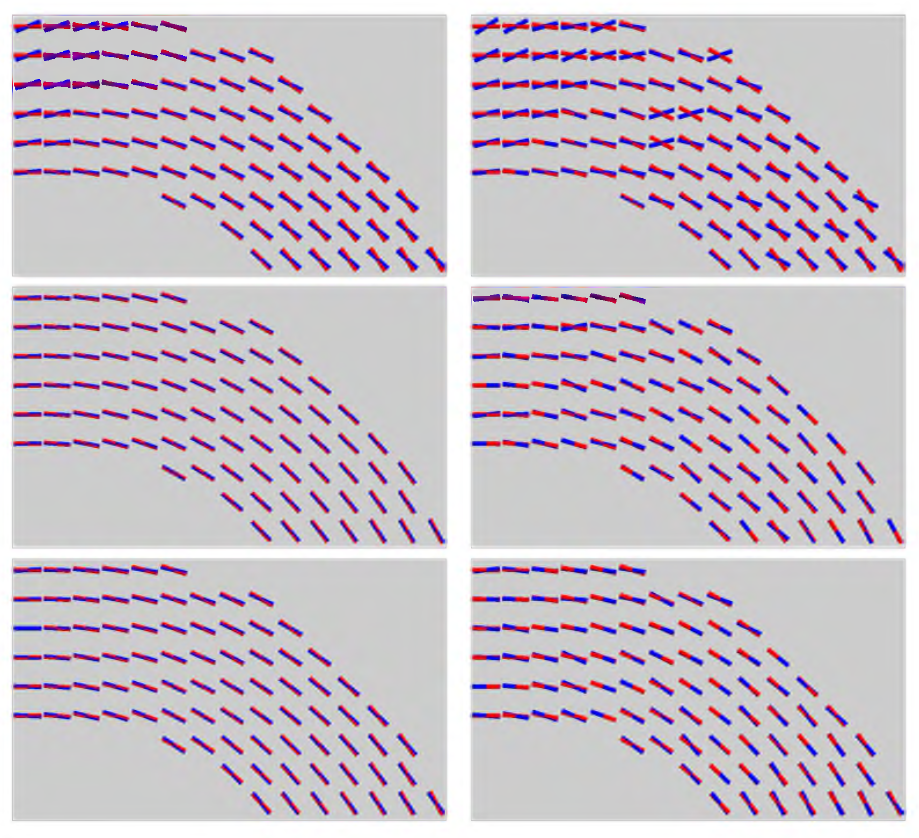
\includegraphics[scale=0.5]{figure/teneigen.png}
    \caption{Tangent vectors of the geodesics (blue) of the generated noise-free data (left column) and noisy data at a SNR of 15 (right column) under the inverse-tensor metric without modulation (top row), sharpened tensor metric (middle row), and with our modulation (bottom row). The red vectors are the principal eigenvectors of the diffusion tensors. We subsample the vector field by a factor of 4 both horizontally and vertically in order to visualize it.}
    % \label{fig:my_label}
\end{figure}

\section{2D Laplace-Beltrami Operator}
$\Delta(u)=\nabla\cdot(g\nabla u)$ is the Laplace-Beltrami operator on $M$, defined as
\begin{equation}
    \Delta(u)=\frac{1}{\sqrt{|g|}}\sum_i\frac{\partial}{\partial x^i}\left(\sqrt{|g|}\sum_j g^{ij}\frac{\partial u}{\partial x^j}\right),
\end{equation}
where $x^i$ is the coordinate basis.
\subsection{Formula Derivation}

$g$ is the Riemannian metric, where $g^{ij}$ denotes the entries of $g$, $g_{ij}$ denotes the entries of $g^{-1}$, namely inverse metric.
\begin{equation}
    g(x^1,x^2)
    =
    \left[\begin{array}{cc}
        g^{11}(x^1,x^2) & g^{12}(x^1,x^2) \\
        g^{21}(x^1,x^2) & g^{22}(x^1,x^2) 
    \end{array}\right], \sqrt{|g|}=\sqrt{g^{11}g^{22}-g^{12}g^{21}}
\end{equation}

Expand Eq.(1), we'll get
\begin{equation}
    \Delta(u)=
    \frac{1}{\sqrt{|g|}}\left[\frac{\partial}{\partial x^1}\sqrt{|g|}\left(g^{11}\frac{\partial u}{\partial x^1}+g^{12}\frac{\partial u}{\partial x^2}\right)+\frac{\partial}{\partial x^2}\sqrt{|g|}\left(g^{21}\frac{\partial u}{\partial x^1}+g^{22}\frac{\partial u}{\partial x^2}\right)\right]
\end{equation}

For continuous one, expanding Eq.(3), we'll get
\begin{align}
    \Delta(u)
    &=\frac{1}{\sqrt{|g|}}\left[\frac{\partial}{\partial x^1}\left(\sqrt{|g|}g^{11}\frac{\partial u}{\partial x^1}+\sqrt{|g|}g^{12}\frac{\partial u}{\partial x^2}\right)+\frac{\partial}{\partial x^2}\left(\sqrt{|g|}g^{12}\frac{\partial u}{\partial x^1}+\sqrt{|g|}g^{22}\frac{\partial u}{\partial x^2}\right)\right]\\ \nonumber
    &=[\frac{\partial \sqrt{|g|}}{\partial x^1}g^{11}\frac{\partial u}{\partial x^1}+\sqrt{|g|}\frac{\partial g^{11}}{\partial x^1}\frac{\partial u}{\partial x^1}+\sqrt{|g|}g^{11}\frac{\partial^2u}{\partial(x^1)^2}\\ \nonumber
    &+\frac{\partial \sqrt{|g|}}{\partial x^1}g^{12}\frac{\partial u}{\partial x^2}+\sqrt{|g|}\frac{\partial g^{12}}{\partial x^1}\frac{\partial u}{\partial x^2}+\sqrt{|g|}g^{12}\frac{\partial^2u}{\partial(x^1)\partial(x^2)}\\ \nonumber
    &+\frac{\partial \sqrt{|g|}}{\partial x^2}g^{12}\frac{\partial u}{\partial x^1}+\sqrt{|g|}\frac{\partial g^{12}}{\partial x^2}\frac{\partial u}{\partial x^1}+\sqrt{|g|}g^{12}\frac{\partial^2u}{\partial(x^1)\partial(x^2)}\\ \nonumber
    &+\frac{\partial \sqrt{|g|}}{\partial x^2}g^{22}\frac{\partial u}{\partial x^2}+\sqrt{|g|}\frac{\partial g^{22}}{\partial x^2}\frac{\partial u}{\partial x^2}+\sqrt{|g|}g^{22}\frac{\partial^2u}{\partial(x^2)^2}]\cdot\frac{1}{\sqrt{|g|}}\\ \nonumber
    &=\frac{\partial \sqrt{|g|}}{\partial x^1}\frac{g^{11}}{\sqrt{|g|}}\frac{\partial u}{\partial x^1}+\frac{\partial g^{11}}{\partial x^1}\frac{\partial u}{\partial x^1}+g^{11}\frac{\partial^2u}{\partial(x^1)^2}\\ \nonumber
    &+\frac{\partial \sqrt{|g|}}{\partial x^1}\frac{g^{12}}{\sqrt{|g|}}\frac{\partial u}{\partial x^2}+\frac{\partial g^{12}}{\partial x^1}\frac{\partial u}{\partial x^2}+g^{12}\frac{\partial^2u}{\partial(x^1)\partial(x^2)}\\ \nonumber
    &+\frac{\partial \sqrt{|g|}}{\partial x^2}\frac{g^{12}}{\sqrt{|g|}}\frac{\partial u}{\partial x^1}+\frac{\partial g^{12}}{\partial x^2}\frac{\partial u}{\partial x^1}+g^{12}\frac{\partial^2u}{\partial(x^1)\partial(x^2)}\\ \nonumber
    &+\frac{\partial \sqrt{|g|}}{\partial x^2}\frac{g^{22}}{\sqrt{|g|}}\frac{\partial u}{\partial x^2}+\frac{\partial g^{22}}{\partial x^2}\frac{\partial u}{\partial x^2}+g^{22}\frac{\partial^2u}{\partial(x^2)^2}\\ \nonumber
    &=\left(\frac{\partial \sqrt{|g|}}{\partial x^1}\frac{g^{11}}{\sqrt{|g|}}+\frac{\partial g^{11}}{\partial x^1}+\frac{\partial \sqrt{|g|}}{\partial x^2}\frac{g^{12}}{\sqrt{|g|}}+\frac{\partial g^{12}}{\partial x^2}\right)\frac{\partial u}{\partial x^1}\\ \nonumber
    &+\left(\frac{\partial \sqrt{|g|}}{\partial x^1}\frac{g^{12}}{\sqrt{|g|}}+\frac{\partial g^{12}}{\partial x^1}+\frac{\partial \sqrt{|g|}}{\partial x^2}\frac{g^{22}}{\sqrt{|g|}}+\frac{\partial g^{22}}{\partial x^2}\right)\frac{\partial u}{\partial x^2}\\ \nonumber
    &+2g^{12}\frac{\partial^2u}{\partial(x^1)\partial(x^2)}+g^{11}\frac{\partial^2u}{\partial(x^1)^2}+g^{22}\frac{\partial^2u}{\partial(x^2)^2}
\end{align}

For discrete function, we can just represent the partial differential terms in Eq.(4) by approximation, as shown in Eq.(5) and Eq.(6).

\begin{align}
    \frac{\partial g^{11}}{\partial x^1}&\approx\frac{1}{2}[g^{11}(x^1+1,x^2)-g^{11}(x^1-1,x^2)]\\ \nonumber
    \frac{\partial g^{12}}{\partial x^1}&\approx\frac{1}{2}[g^{12}(x^1+1,x^2)-g^{12}(x^1-1,x^2)]\\ \nonumber
    \frac{\partial g^{12}}{\partial x^2}&\approx\frac{1}{2}[g^{12}(x^1,x^2+1)-g^{12}(x^1,x^2-1)]\\ \nonumber
    \frac{\partial g^{22}}{\partial x^2}&\approx\frac{1}{2}[g^{22}(x^1,x^2+1)-g^{22}(x^1,x^2-1)]\\ \nonumber
    \frac{\partial \sqrt{|g|}}{\partial x^1}&\approx\frac{1}{2}[\sqrt{|g|}(x^1+1,x^2)-\sqrt{|g|}(x^1-1,x^2)]\\ \nonumber
    \frac{\partial \sqrt{|g|}}{\partial x^2}&\approx\frac{1}{2}[\sqrt{|g|}(x^1,x^2+1)-\sqrt{|g|}(x^1,x^2-1)]
\end{align}

\begin{align}
    \frac{\partial u}{\partial x^1}&\approx \frac{1}{2}[u(x^1+1,x^2)-u(x^1-1,x^2)]\\ \nonumber
    \frac{\partial u}{\partial x^2}&\approx \frac{1}{2}[u(x^1,x^2+1)-u(x^1,x^2-1)]\\ \nonumber
    \frac{\partial^2 u}{\partial (x^1)^2}&\approx u(x^1+1,x^2)+u(x^1-1,x^2)-2u(x^1,x^2)\\ \nonumber
    \frac{\partial^2 u}{\partial (x^2)^2}&\approx u(x^1,x^2+1)+u(x^1,x^2-1)-2u(x^1,x^2)\\ \nonumber
    \frac{\partial^2 u}{\partial x^1\partial x^2}&\approx \frac{1}{2}[u(x^1+1,x^2+1)+u(x^1-1,x^2-1)-u(x^1+1,x^2-1)-u(x^1-1,x^2+1)]
\end{align}

Therefore, the value at $(x^1,x^2)$ after the operation can be represent as two vectors' inner product.
\begin{equation}
    \Delta(u) =<\vec{e},\vec{u}>
\end{equation}

And $\vec{e}$ and $\vec{u}$ can be written as Eq.(8), after simplification.
\begin{equation}
    \vec e=\left[
    \begin{array}{cc}
         e_1\\
         e_2\\
         e_3\\
         e_4\\
         e_5\\
         e_6\\
         e_7\\
         e_8\\
         e_9
    \end{array}
    \right]=\left[
    \begin{array}{cc}
         \frac{\partial \sqrt{|g|}}{\partial x^1}\frac{g^{11}}{\sqrt{|g|}}+\frac{\partial g^{11}}{\partial x^1}+\frac{\partial \sqrt{|g|}}{\partial x^2}\frac{g^{12}}{\sqrt{|g|}}+\frac{\partial g^{12}}{\partial x^2}+2g_{11}\\
         -\frac{\partial \sqrt{|g|}}{\partial x^1}\frac{g^{11}}{\sqrt{|g|}}-\frac{\partial g^{11}}{\partial x^1}-\frac{\partial \sqrt{|g|}}{\partial x^2}\frac{g^{12}}{\sqrt{|g|}}-\frac{\partial g^{12}}{\partial x^2}+2g_{11}\\
         2g^{12}\\
         -2g^{12}\\
         -4g^{11}-4g^{22}\\
         -2g^{12}\\
         2g^{12}\\
         -\frac{\partial \sqrt{|g|}}{\partial x^1}\frac{g^{12}}{\sqrt{|g|}}-\frac{\partial g^{12}}{\partial x^1}-\frac{\partial \sqrt{|g|}}{\partial x^2}\frac{g^{22}}{\sqrt{|g|}}-\frac{\partial g^{22}}{\partial x^2}+2g_{22}\\
         \frac{\partial \sqrt{|g|}}{\partial x^1}\frac{g^{12}}{\sqrt{|g|}}+\frac{\partial g^{12}}{\partial x^1}+\frac{\partial \sqrt{|g|}}{\partial x^2}\frac{g^{22}}{\sqrt{|g|}}+\frac{\partial g^{22}}{\partial x^2}+2g_{22}\\
    \end{array}
    \right],
    \vec u=\frac{1}{2}\left[
    \begin{array}{cc}
         u(x^1+1,x^2)  \\
         u(x^1-1,x^2)   \\
         u(x^1+1,x^2+1)  \\
         u(x^1+1,x^2-1)   \\
         u(x^1,x^2)   \\
         u(x^1-1,x^2+1)   \\
         u(x^1-1,x^2-1)   \\
         u(x^1,x^2-1) \\
         u(x^1,x^2+1)  
    \end{array}
    \right]
\end{equation}
Eq.(9) shows $\vec{e}$ 's every components in the form of $ g$:

\begin{align}
    e_1&\approx\frac{1}{2}(\sqrt{g}(x^1+1,x^2)-\sqrt{g}(x^1-1,x^2))\cdot\frac{g^{11}}{\sqrt{g}}+\frac{1}{2}(g^{11}(x^1+1,x^2)-g^{11}(x^1-1,x^2))\\ \nonumber
    &+\frac{1}{2}(\sqrt{g}(x^1,x^2+1)-\sqrt{g}(x^1,x^2-1))\cdot\frac{g^{12}}{\sqrt{g}}+\frac{1}{2}(g^{12}(x^1,x^2+1)-g^{12}(x^1,x^2-1))+2g^{11}\\ \nonumber
    e_2&\approx-\frac{1}{2}(\sqrt{g}(x^1+1,x^2)-\sqrt{g}(x^1-1,x^2))\cdot\frac{g^{11}}{\sqrt{g}}-\frac{1}{2}(g^{11}(x^1+1,x^2)-g^{11}(x^1-1,x^2))\\ \nonumber
    &-\frac{1}{2}(\sqrt{g}(x^1,x^2+1)-\sqrt{g}(x^1,x^2-1))\cdot\frac{g^{12}}{\sqrt{g}}-\frac{1}{2}(g^{12}(x^1,x^2+1)-g^{12}(x^1,x^2-1))+2g^{11}\\ \nonumber
    e_3&=2 g^{12}\\ \nonumber
    e_4&=-2 g^{12}\\ \nonumber
    e_5&=-4 g^{11}-4 g^{22}\\ \nonumber
    e_6&=-2 g^{12}\\ \nonumber
    e_7&=2 g^{12}\\ \nonumber
    e_8&\approx-\frac{1}{2}(\sqrt{g}(x^1+1,x^2)-\sqrt{g}(x^1-1,x^2))\cdot\frac{g^{12}}{\sqrt{g}}-\frac{1}{2}(g^{12}(x^1+1,x^2)-g^{12}(x^1-1,x^2))\\ \nonumber
    &-\frac{1}{2}(\sqrt{g}(x^1,x^2+1)-\sqrt{g}(x^1,x^2-1))\cdot\frac{g^{22}}{\sqrt{g}}-\frac{1}{2}(g^{22}(x^1,x^2+1)-g^{22}(x^1,x^2-1))+2g^{22}\\ \nonumber
    e_9&\approx\frac{1}{2}(\sqrt{g}(x^1+1,x^2)-\sqrt{g}(x^1-1,x^2))\cdot\frac{g^{12}}{\sqrt{g}}+\frac{1}{2}(g^{12}(x^1+1,x^2)-g^{12}(x^1-1,x^2))\\ \nonumber
    &+\frac{1}{2}(\sqrt{g}(x^1,x^2+1)-\sqrt{g}(x^1,x^2-1))\cdot\frac{g^{22}}{\sqrt{g}}+\frac{1}{2}(g^{22}(x^1,x^2+1)-g^{22}(x^1,x^2-1))+2g^{22}\\
\end{align}
Finally, with $\vec{e}$ in the form of $g$, we'll obtain a more specific expression of  $\Delta(u)=\nabla\cdot(g\nabla u)$.


\section{Calculating Scaling Field for Adaptive Riemannian Metrics\cite{hao2011adaptive}}
\subsection{Using Inverse Tensor Field as the Metric}
We want to find a metric $\bar{g}=e^{2\alpha}g$ on $M$ such that
\begin{equation}
    \bar{\nabla}_VV=\vec{0}
\end{equation}

$\nabla_XY$ is the affine connection
\begin{align}
    \nabla_XY&=\sum_k^n\left(\sum_i a^i\frac{\partial b^k}{\partial x^i}+\sum_{i,j}\Gamma_{ij}^k a^i b^j\right)\vec{E_k},\\ \nonumber
    \Gamma_{ij}^k&=\frac{1}{2}\sum_{l}^n  g^{kl}\left(\frac{\partial  g_{jl}}{\partial x^i}+\frac{\partial  g_{il}}{\partial x^j}-\frac{\partial  g_{ij}}{\partial x^l}\right),
\end{align}
where $n$ is the dimension of the vector field $X,Y$ and $\vec{E_k}=\frac{\partial}{\partial x^k}$ are the basis vectors. So basically, $\nabla_XY$ is a vector field. $\bar{\nabla}, \bar{\Gamma}^k_{ij}$ are the affine connection and the Christoffel symbols with respect to $\bar{g}$. To be more specifical, we can have the $\bar{\Gamma}$ expressed as below
\begin{align}
    \bar{\Gamma}^k_{ij} &= \frac12g^{kl}\left(\partial_i\bar{g}_{lj} + \partial_j\bar{g}_{il}  - \partial_l\bar{g}_{ij}\right) \\ \nonumber
	&=\frac12 e^{-2\alpha}g^{kl}(\partial_i(e^{2\alpha}g_{lj})+\partial_j(e^{2\alpha}g_{il})-\partial_l(e^{2\alpha}g_{ij}))\\ \nonumber
	&=\frac12 e^{-2\alpha}g^{kl}(g_{lj}\partial_ie^{2\alpha}+e^{2\alpha}\partial_ig_{lj}+g_{il}\partial_je^{2\alpha}+e^{2\alpha}\partial_jg_{il}-g_{ij}\partial_le^{2\alpha}-e^{2\alpha}\partial_lg_{ij})\\ \nonumber
	&=\frac12 e^{-2\alpha}g^{kl}(g_{lj}\partial_ie^{2\alpha}+g_{il}\partial_je^{2\alpha}-g_{ij}\partial_le^{2\alpha}+e^{2\alpha}\partial_ig_{lj}+e^{2\alpha}\partial_jg_{il}-e^{2\alpha}\partial_lg_{ij})\\ \nonumber
	&=g^{kl}[g_{lj}\partial_i\alpha+g_{il}\partial_j\alpha-g_{ij}\partial_l\alpha]+\frac{1}{2}g^{kl}[\partial_ig_{lj}+\partial_jg_{il}-\partial_lg_{ij}]\\ \nonumber
	&\text{Since $g$ is the Euclidean metric, we can have the final expression}\\ \nonumber
	&=\delta^k_l\partial_i\alpha+\delta^k_i\partial_j\alpha-g_{ij}g^{kl}\partial_l\alpha+\Gamma^k_{ij}
\end{align}
Substituting Eq.(13) into Eq.(11), we then obtain
\begin{equation}
    v^j\partial_jv^k+(\delta^k_l\partial_i\alpha+\delta^k_i\partial_j\alpha-g_{ij}g^{kl}\partial_l\alpha+\Gamma^k_{ij})v^iv^j=\vec{0}
\end{equation}
which can be simplified further as 
\begin{align}
    \nabla_VV+2\nabla_V(\alpha)V-\nabla\alpha&=0\\ \nonumber
    2<\nabla_v(\alpha)V,V>_g-<\nabla\alpha,V>_g&=0\\ \nonumber
    \nabla\alpha&=\nabla_VV
\end{align}
Let $X=Y=V$, expand the $\nabla_VV$ expression completely, we can have
\begin{align}
    \nabla_V V&=\left[\begin{array}{c}
        v^1\partial_1 v^1+v^2\partial_2 v^1+\Gamma_{11}^1v^1v^1+\Gamma_{12}^1v^1v^2+\Gamma_{21}^1v^2v^1+\Gamma_{22}^1v^2v^2 \\
        v^1\partial_1 v^2+v^2\partial_2 v^2+\Gamma_{11}^2v^1v^1+\Gamma_{12}^2v^1v^2+\Gamma_{21}^2v^2v^1+\Gamma_{22}^2v^2v^2
    \end{array}\right]\\ \nonumber
    &=
    \left[\begin{array}{c}
    v^1\partial_1 v^1+v^2\partial_2 v^1+\Gamma_{11}^1v^1v^1+2\Gamma_{12}^1v^1v^2+\Gamma_{22}^1v^2v^2\\
    v^1\partial_1 v^2+v^2\partial_2 v^2+\Gamma_{11}^2v^1v^1+2\Gamma_{12}^2v^1v^2+\Gamma_{22}^2v^2v^2
    \end{array}\right]
\end{align}
To be more specific, the Christoffel symbol $\Gamma_{ij}^k$ in 2D space would be
\begin{align}
    \Gamma_{11}^1=\frac{1}{2}\left[ g^{11}\left(\frac{\partial  g_{11}}{\partial x^1}+\frac{\partial  g_{11}}{\partial x^1}-\frac{\partial  g_{11}}{\partial x^1}\right)+ g^{12}\left(\frac{\partial  g_{12}}{\partial x^1}+\frac{\partial  g_{12}}{\partial x^1}-\frac{\partial  g_{11}}{\partial x^2}\right)\right]\\ \nonumber
    \Gamma_{12}^1=\frac{1}{2}\left[ g^{11}\left(\frac{\partial  g_{21}}{\partial x^1}+\frac{\partial  g_{11}}{\partial x^2}-\frac{\partial  g_{12}}{\partial x^1}\right)+ g^{12}\left(\frac{\partial  g_{22}}{\partial x^1}+\frac{\partial  g_{12}}{\partial x^2}-\frac{\partial  g_{12}}{\partial x^2}\right)\right]\\ \nonumber
    \Gamma_{21}^1=\frac{1}{2}\left[ g^{11}\left(\frac{\partial  g_{11}}{\partial x^2}+\frac{\partial  g_{21}}{\partial x^1}-\frac{\partial  g_{21}}{\partial x^1}\right)+ g^{12}\left(\frac{\partial  g_{12}}{\partial x^2}+\frac{\partial  g_{22}}{\partial x^1}-\frac{\partial  g_{21}}{\partial x^2}\right)\right]\\ \nonumber
    \Gamma_{22}^1=\frac{1}{2}\left[ g^{11}\left(\frac{\partial  g_{21}}{\partial x^2}+\frac{\partial  g_{21}}{\partial x^2}-\frac{\partial  g_{22}}{\partial x^1}\right)+ g^{12}\left(\frac{\partial  g_{22}}{\partial x^2}+\frac{\partial  g_{22}}{\partial x^2}-\frac{\partial  g_{22}}{\partial x^2}\right)\right]\\ \nonumber
    \Gamma_{11}^2=\frac{1}{2}\left[ g^{21}\left(\frac{\partial  g_{11}}{\partial x^1}+\frac{\partial  g_{11}}{\partial x^1}-\frac{\partial  g_{11}}{\partial x^1}\right)+ g^{22}\left(\frac{\partial  g_{12}}{\partial x^1}+\frac{\partial  g_{12}}{\partial x^1}-\frac{\partial  g_{11}}{\partial x^2}\right)\right]\\ \nonumber
    \Gamma_{12}^2=\frac{1}{2}\left[ g^{21}\left(\frac{\partial  g_{21}}{\partial x^1}+\frac{\partial  g_{11}}{\partial x^2}-\frac{\partial  g_{12}}{\partial x^1}\right)+ g^{22}\left(\frac{\partial  g_{22}}{\partial x^1}+\frac{\partial  g_{12}}{\partial x^2}-\frac{\partial  g_{12}}{\partial x^2}\right)\right]\\ \nonumber
    \Gamma_{21}^2=\frac{1}{2}\left[ g^{21}\left(\frac{\partial  g_{11}}{\partial x^2}+\frac{\partial  g_{21}}{\partial x^1}-\frac{\partial  g_{21}}{\partial x^1}\right)+ g^{22}\left(\frac{\partial  g_{12}}{\partial x^2}+\frac{\partial  g_{22}}{\partial x^1}-\frac{\partial  g_{21}}{\partial x^2}\right)\right]\\ \nonumber
    \Gamma_{22}^2=\frac{1}{2}\left[ g^{21}\left(\frac{\partial  g_{21}}{\partial x^2}+\frac{\partial  g_{21}}{\partial x^2}-\frac{\partial  g_{22}}{\partial x^1}\right)+ g^{22}\left(\frac{\partial  g_{22}}{\partial x^2}+\frac{\partial  g_{22}}{\partial x^2}-\frac{\partial  g_{22}}{\partial x^2}\right)\right]
\end{align}
where $g$ is the metric, and the Christoffel symbols are only related to the metric. 

While, the relationship between $ g$ with subscript and superscript is
\begin{equation}
    \left[\begin{array}{cc}
         g_{11} &  g_{12} \\
         g_{21} &  g_{22}
    \end{array}\right]
    =
    \left[\begin{array}{cc}
         g^{11} &  g^{12} \\
         g^{21} &  g^{22}
    \end{array}\right]^{-1}=g^{-1}
\end{equation}

If the original $g$ is an Euclidean metric, then all the Christoffel symbols above will equal to 0. 
\begin{align}
    \nabla_V V&=
    \left[\begin{array}{c}
    v^1\partial_1 v^1+v^2\partial_2 v^1\\
    v^1\partial_1 v^2+v^2\partial_2 v^2
    \end{array}\right]
\end{align}

However, the metric we use here is not Euclidean metric, so the $\nabla_VV$ is still like
Eq.(16).

The $\alpha$ satisfies the equation that $\Delta \alpha={\rm div}(\nabla_VV)$ is the scaling field we want.\\

\subsection{Conformal Simple Metric}
If we want to find conformally flat metric
\begin{equation}
    \bar{g}=\left[\begin{array}{cc}
         e^{2\alpha} &  0 \\
         0 &  e^{2\alpha}
    \end{array}\right], 
    \bar{g}^{-1}=\left[\begin{array}{cc}
         e^{-2\alpha} &  0 \\
         0 &  e^{-2\alpha}
    \end{array}\right]
\end{equation}

We can yield the respective Christoffel symbols as below
\begin{align}
    \bar{\Gamma}^k_{ij} &= \frac12g^{kl}\left(\partial_i\bar{g}_{lj} + \partial_j\bar{g}_{il}  - \partial_l\bar{g}_{ij}\right) \\ \nonumber
	&=\frac12 e^{-2\alpha}\delta^{kl}\left(\delta_{lj}\partial_ie^{2\alpha}+e^{2\alpha}\partial_i\delta_{lj}+ \delta_{il}\partial_je^{2\alpha}+ e^{2\alpha}\partial_j \delta_{il}- \delta_{ij}\partial_le^{2\alpha}-e^{2\alpha}\partial_l\delta_{ij}\right)\\ \nonumber
	&=\frac12 e^{-2\alpha}\delta^{kl}\left(\delta_{lj}\partial_ie^{2\alpha} + \delta_{il}\partial_je^{2\alpha} - \delta_{ij}\partial_le^{2\alpha} \right)\\ \nonumber
	&=\delta^{kl}\left(\delta_{lj}\partial_i\alpha + \delta_{il}\partial_j\alpha - \delta_{ij}\partial_l\alpha\right)\\ \nonumber
	&=\delta^k_j\partial_i\alpha + \delta^k_i\partial_j\alpha - \delta_{ij}\partial_k\alpha.
\end{align}

Further more, we can have the simplified expressions of the Christoffel symbols:
\begin{align}
	&\bar{\Gamma}^1_{11} = \partial_1\alpha,\quad \bar{\Gamma}^1_{12} = \bar{\Gamma}^1_{21} = \partial_2\alpha,\quad 
	\bar{\Gamma}^1_{22} = -\partial_1\alpha \\ \nonumber
	&\bar{\Gamma}^2_{11} = -\partial_2\alpha,\quad \bar{\Gamma}^2_{12} = \bar{\Gamma}^2_{21} = \partial_1\alpha,\quad 
	\bar{\Gamma}^2_{22} = \partial_2\alpha.  
\end{align}

What we want is in the metric $\bar{g}$, every integral curve of $V$ is a geodesic, which is equivalent to say that $\nabla_VV=\vec{0}$.
\begin{equation}
    \nabla_V V=
    \left[\begin{array}{c}
    v^1\partial_1 v^1+v^2\partial_2 v^1+\bar{\Gamma}_{11}^1v^1v^1+\bar{\Gamma}_{12}^1v^1v^2+\bar{\Gamma}_{21}^1v^2v^1+\bar{\Gamma}_{22}^1v^2v^2 \\
    v^1\partial_1 v^2+v^2\partial_2 v^2+\bar{\Gamma}_{11}^2v^1v^1+\bar{\Gamma}_{12}^2v^1v^2+\bar{\Gamma}_{21}^2v^2v^1+\bar{\Gamma}_{22}^2v^2v^2
    \end{array}\right]
    =
    \left[\begin{array}{c}
    0 \\
    0
    \end{array}\right]
\end{equation}

Substituting the given Christoffel symbols in Eq.(22) into Eq.(24), we can yield 
\begin{align}
	\left(v^1v^1 - v^2v^2\right)\partial_1\alpha + 2v^1v^2\partial_2\alpha+v^1\partial_1v^1 + v^2\partial_2v^1 &= 0\\ \nonumber
	2v^1v^2\partial_1\alpha +\left(v^2v^2 - v^1v^1\right)\partial_2\alpha+v^1\partial_1v^2+v^2\partial_2v^2&= 0
\end{align}

Finally, we get
\begin{align}
	\left[\begin{array}{c}
	\partial_1\alpha\\
	\partial_2\alpha
	\end{array}\right]&= \frac{-1}{(v^1v^1 + v^2v^2)^2}
	\left[\begin{array}{cc}
	v^1v^1 - v^2v^2 & 2v^1v^2\\
	2v^1v^2 & v^2v^2-v^1v^1
	\end{array}\right]
	\left[\begin{array}{cc}
	\partial_1v^1 & \partial_2v^1\\
	\partial_1v^2 & \partial_2v^2
	\end{array}\right]
	\left[\begin{array}{c}
	v^1\\
	v^2
	\end{array}\right]\notag\\
	&=\frac{-1}{(v^1v^1 + v^2v^2)^2}
	\left[\begin{array}{cc}
	v^1  & -v^2\\
	v^2 & v^1
	\end{array}\right]
	\left[\begin{array}{cc}
	v^1  & v^2\\
	v^2 & -v^1
	\end{array}\right]
	\left[\begin{array}{cc}
	\partial_1v^1 & \partial_2v^1\\
	\partial_1v^2 & \partial_2v^2
	\end{array}\right]
	\left[\begin{array}{c}
	v^1\\
	v^2
	\end{array}\right]
\end{align}

The ${\rm div}$ operator used below is the Riemannian divergence, and the divergence of $V$ on $M$ is defined in coordinates as
\begin{equation}
    {\rm div}(V)=\frac{1}{\sqrt{|g|}}\sum_i\frac{\partial}{\partial v^i}(\sqrt{|g|}a^i),
\end{equation}
where $a^i$ is the corresponding component of vector field $V$. The metric $g$ used is also the original Euclidean metric.

\subsection{Geodesics and Christoffel Symbol}
In curved space, a straight path has zero tangential acceleration when we travel along it at constant speed. To compute geodesic curves, we need to find curves where the acceleration vector is normal to the space.
In this section, all the computations are conducted in 2D situation.
\begin{align}
    \text{Velocity Vector:}&&\frac{d\vec{R}}{dt}=\frac{\partial\vec{R}}{\partial u}\cdot\frac{du}{dt}+\frac{\partial\vec{R}}{\partial v}\cdot\frac{dv}{dt}\\
    \text{Acceleration Vector:}&&\frac{d^2\vec{R}}{dt^2}=\frac{d}{dt}\left(\frac{\partial\vec{R}}{\partial u}\cdot\frac{du}{dt}+\frac{\partial\vec{R}}{\partial v}\cdot\frac{dv}{dt}\right)
\end{align}
\begin{equation}
    \frac{d^2\vec{R}}{d t^2}=\frac{d^2 u}{d t^2}\cdot\frac{\partial \vec{R}}{\partial u}+\frac{d^2 v}{d t^2}\cdot\frac{\partial \vec{R}}{\partial v}+\left(\frac{du}{dt}\right)^2\cdot\frac{\partial^2\vec{R}}{\partial u^2}+\left(\frac{dv}{dt}\right)^2\cdot\frac{\partial^2\vec{R}}{\partial v^2}+\frac{du}{dt}\cdot\frac{dv}{dt}\cdot\frac{\partial^2\vec{R}}{\partial u\partial v}+\frac{dv}{dt}\cdot\frac{du}{dt}\cdot\frac{\partial^2\vec{R}}{\partial u\partial v}
\end{equation}

By using Einstein Notation, and making $x^1=u, x^2=v$, we can denote the acceleration vector like 
\begin{equation}
    \frac{d^2\vec{R}}{d t^2}=\frac{d^2 x^i}{d t^2}\cdot\frac{\partial \vec{R}}{\partial x^i}+\frac{dx^i}{dt}\cdot\frac{dx^j}{dt}\cdot\frac{\partial^2\vec{R}}{\partial x^i\partial x^j}
\end{equation}

Assuming that $\frac{\partial^2\vec{R}}{\partial x^i\partial x^j}$ is consist of three components, so we can express it like
\begin{equation}
    \frac{\partial^2\vec{R}}{\partial x^i\partial x^j}=\Gamma_{ij}^1\frac{\partial \vec{R}}{\partial x^1}+\Gamma_{ij}^2\frac{\partial \vec{R}}{\partial x^2}+L_{ij}\vec{n}
\end{equation}
where the Christoffel symbol $\Gamma_{ij}^k$, gives us the tangential component of $\frac{\partial^2\vec{R}}{\partial x^i\partial x^j}$ and the second fundamental form $L_{ij}$, gives us the normal components of $\frac{\partial^2\vec{R}}{\partial x^i \partial x^j}$.\\
Also by using Einstein Notation, we can have a more concise form of $\frac{\partial^2\vec{R}}{\partial x^i\partial x^j}$.
\begin{equation}
    \frac{\partial^2\vec{R}}{\partial x^i\partial x^j}=\Gamma_{ij}^k\frac{\partial \vec{R}}{\partial x^k}+L_{ij}\vec{n}
\end{equation}

As $\vec{n}$ is perpendicular to the tangent vectors, therefore, by multiplying $\frac{\vec{R}}{\partial x^l}$ on both side of Eq.(33), we can yield that
\begin{equation}
    \frac{\partial^2\vec{R}}{\partial x^i\partial x^j}\cdot\frac{\partial\vec{R}}{\partial x^l}=\left(\Gamma_{ij}^k\frac{\partial \vec{R}}{\partial x^k}+L_{ij}\vec{n}\right)\cdot\frac{\partial\vec{R}}{\partial x^l}=\Gamma_{ij}^k\frac{\partial \vec{R}}{\partial x^k}\cdot\frac{\partial\vec{R}}{\partial x^l}
\end{equation}

Since intrinsic metric tensor is
\begin{equation}
    \left[\begin{array}{cc}
        \frac{\partial\vec{R}}{\partial x^1}\cdot\frac{\partial\vec{R}}{\partial x^1} & \frac{\partial\vec{R}}{\partial x^1}\cdot\frac{\partial\vec{R}}{\partial x^2} \\
        \frac{\partial\vec{R}}{\partial x^2}\cdot\frac{\partial\vec{R}}{\partial x^1} & \frac{\partial\vec{R}}{\partial x^2}\cdot\frac{\partial\vec{R}}{\partial x^2}
    \end{array}\right]
    =
    \left[\begin{array}{cc}
        g_{11} & g_{12} \\
        g_{21} & g_{22}
    \end{array}\right],
\end{equation}
we can rewrite Eq.(34) by substituting $\frac{\partial \vec{R}}{\partial x^k}\cdot\frac{\partial\vec{R}}{\partial x^l}$ with $g_{kl}$. Then we get
\begin{equation}
    \frac{\partial^2\vec{R}}{\partial x^i\partial x^j}\cdot\frac{\partial\vec{R}}{\partial x^l}=\Gamma_{ij}^kg_{kl}
\end{equation}

The summation of metric tensor components with the inverse metric tensor components gives us the Kronecker delta
\begin{equation}
    g_{kl}\cdot g^{lm}=\delta_k^m
\end{equation}

Therefore, with Kronecker delta cancellation rule, we can have
\begin{equation}
    \frac{\partial^2\vec{R}}{\partial x^i\partial x^j}\cdot\frac{\partial\vec{R}}{\partial x^l}\cdot g^{lm}=\Gamma_{ij}^kg_{kl}g^{lm}=\Gamma_{ij}^k\delta_k^m=\Gamma_{ij}^m
\end{equation}

We get the final expression of Christoffel symbol like below
\begin{equation}
    \boxed{\Gamma_{ij}^k=\frac{\partial^2\vec{R}}{\partial x^i\partial x^j}\cdot\frac{\partial\vec{R}}{\partial x^l}\cdot g^{lk}}
\end{equation}

Likewise, by multiplying $\vec{n}$ at both side of Eq.(33), we can yield the final expression of second fundamental form
\begin{equation}
    \boxed{L_{ij}=\frac{\partial^2\vec{R}}{\partial x^i\partial x^j}\cdot \vec{n}}
\end{equation}

Finally, we can have acceleration vector like this
\begin{equation}
    \frac{d^2\vec{R}}{dt^2}=\underbrace{\left(\frac{d^2x^k}{dt^2}+\Gamma_{ij}^k\frac{dx^i}{dt}\cdot\frac{dx^j}{dt}\right)\frac{\partial\vec{R}}{\partial x^k}}_{\text{tangential part}}+\underbrace{L_{ij}\cdot\frac{dx^i}{dt}\cdot\frac{dx^j}{dt}\cdot\vec{n}}_{\text{normal part}}
\end{equation}

To make the acceleration vector normal to the surface, we need to make
\begin{equation}
    \boxed{\frac{d^2x^k}{dt^2}+\Gamma_{ij}^k\frac{dx^i}{dt}\cdot\frac{dx^j}{dt}=0},
\end{equation}
which is namely Geodesic Equation.

\subsection{Dijkstra}
\begin{figure}[H]
   \centering
   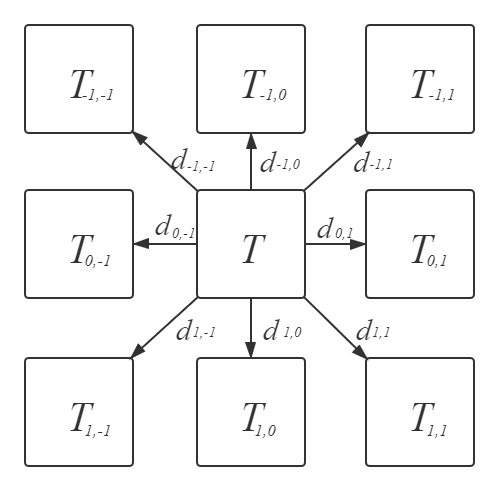
\includegraphics[scale=0.5]{figure/dijkstra.png}
   \caption{edge distance to the neighbors}
\end{figure}

\begin{equation}
    |d_{ij}|=\langle[i,j],\left(\frac{T+T_{ij}}{2}\right)^{-1}[i,j]^T\rangle
\end{equation}
where $T$ is the tensor, while $T_{ij}$ is the neighbor tensor with respect to $T$ and $d_{ij}$ is the distance to the neighbor tensor $T_{ij}$. By doing this, we can have a huge graph, on where we can implement Dijkstra to find the shortest path between two given tensors.

\subsection{Geodesic Shooting(Euler Method)}
$\gamma(t), \Dot{\gamma(t)}, \Ddot{\gamma(t)}$ are the position vector, velocity vector and acceleration vector, respectively, where
\begin{equation}
    \Ddot{\gamma}(t)=F(\gamma(t),\Dot{\gamma}(t))
\end{equation}
\begin{equation}
    \gamma(t)=\left[\begin{array}{c}
         \gamma_1(t) \\
         \gamma_2(t)
    \end{array}\right],
    \Dot{\gamma}(t)=\left[\begin{array}{c}
         \frac{\partial \gamma_1(t)}{\partial t} \\
         \frac{\partial \gamma_2(t)}{\partial t}
    \end{array}\right],
    \Ddot{\gamma}(t)=\left[\begin{array}{c}
         \frac{\partial^2\gamma_1(t)}{\partial t^2} \\
         \frac{\partial^2\gamma_2(t)}{\partial t^2}
    \end{array}\right]
\end{equation}
Explicitly, the $\Ddot{\gamma}(t)$'s corresponding components can be expressed by Eq.(47), where the $u, v, w\in\{1,2\}$, representing the two base directions in 2D space.
\begin{align}
    \Ddot{\gamma_w}(t)&=-\sum_u\sum_v\Gamma^w_{uv}\frac{d\gamma_u(t)}{dt}\frac{d\gamma_v(t)}{dt}\\ \nonumber
    &=-\sum_u\sum_v\Gamma^w_{uv}\Dot{\gamma}_u(t)\Dot{\gamma}_v(t)
\end{align}
More specifically, the acceleration vector's two components (distinguished by subscript) can be written in matrix form, as Eq.(48) and Eq.(49) show.
\begin{equation}
    \Ddot{\gamma}_1(t)=-\left[\begin{array}{cc}\Dot{\gamma}_1(t) & \Dot{\gamma}_2(t)\end{array}\right]
    \left[\begin{array}{cc}
        \Gamma^1_{11} & \Gamma^1_{12} \\
        \Gamma^1_{21} & \Gamma^1_{22}
    \end{array}\right]
    \left[\begin{array}{c}
         \Dot{\gamma}_1(t) \\
         \Dot{\gamma}_2(t)
    \end{array}\right]
\end{equation}

\begin{equation}
    \Ddot{\gamma}_2(t)=-\left[\begin{array}{cc}\Dot{\gamma}_1(t) & \Dot{\gamma}_2(t)\end{array}\right]
    \left[\begin{array}{cc}
        \Gamma^2_{11} & \Gamma^2_{12} \\
        \Gamma^2_{21} & \Gamma^2_{22}
    \end{array}\right]
    \left[\begin{array}{c}
         \Dot{\gamma}_1(t) \\
         \Dot{\gamma}_2(t)
    \end{array}\right]
\end{equation}
The update rules are given below.
\begin{align}
    \gamma(t+\Delta t)&=\gamma(t)+\Delta t\cdot\Dot{\gamma}(t)\\ \nonumber
    \Dot{\gamma}(t+\Delta t)&=\Dot{\gamma}(t)+\Delta t\cdot\Ddot{\gamma}(t)
\end{align}

The algorithm below illustrate the process more specifically.
\begin{algorithm}  
\caption{Geodesic Integrating}\label{algo6}
    \begin{algorithmic}
        \State $\Dot{\gamma}(0)=\text{principal eigenvector at }\gamma(0)$
        \State $\gamma(1)=\gamma(0)+\epsilon\Dot{\gamma}(0)$
        \For{$t=2:iternum$}
            \State $\Ddot{\gamma}_1(t-2)=Eq.48$\Comment{1st component of $\Ddot{\gamma}(t-2)$}
            \State $\Ddot{\gamma}_2(t-2)=Eq.49$\Comment{2nd component of $\Ddot{\gamma}(t-2)$}
            \State $\Dot{\gamma}(t-1)=\Dot{\gamma}(t-2)+\epsilon_1\Ddot{\gamma}(t-2)$
            \State $\gamma(t)=\gamma(t-1)+\epsilon_2\Dot{\gamma}(t-1)$
        \EndFor
        \State \Return{$\gamma$}
    \end{algorithmic}  
\end{algorithm}  
\section{Loss Function}
\begin{align*}
    f(x)&=(Ax-b)^2\\
    &=(Ax-b)^T(Ax-b)\\
    &=(x^TA^T-b^T)(Ax-b)\\
    &=x^TA^TAx-b^TAx-x^TA^Tb+b^Tb\\
    \nabla f(x)&=A^TAx-A^Tb
\end{align*}
\renewcommand\refname{Reference}
\bibliographystyle{plain}
\bibliography{reference}
\end{document}
